\section{MiniMax-Algorithmus}

MiniMax ist ein Algorithmus f�r rundenbasierte Nullsummenspiele. Bei diesem Algorithmus \textbf{maximiert} Spieler A seine Gewinnchancen, wobei er davon ausgeht, dass Spieler B versuchen wird, die Gewinnchancen von Spieler A zu \textbf{minimieren}.

\subsection{Ablauf des MiniMax-Algorithmus}

Der Algorithmus l�uft wie folgt ab:

\begin{enumerate}
    \item Erzeuge eines Suchbaums, wobei die Wurzel die Startposition des Spiels ist und das Ende des Baums die m�glichen Endzust�nde des Spiels darstellt.
    \item Berechne die Gewinnchancen f�r Spieler A f�r jeden Zweig von den Endzust�nden zur�ck zum Ursprung berechnet.
    \item F�r jede Ebene im Suchbaum berechne der Wert f�r die Gewinnchancen von A eines Knotens aus den Werten seiner Nachfolgeknoten. Falls Spieler A am Zug ist, dann ist der Knotenwert der Maximum der Nachfolger, und falls Spieler B am Zug ist, dann ist der Knotenwert der Minimum der Nachfolger.
    \item Nachdem alle Knoten berechnet wurden, w�hlt Spieler A den Weg, der ihm am meisten n�tzt.
\end{enumerate}

Dies l�sst sich am besten anhand eines einfachen Spiels namens ``Nimm'' demonstrieren (siehe Abb. \ref{fig:minmax-nimm-example}). In diesem Spiel gibt es n Objekte. Die Spieler entfernen abwechselnd 1, 2 oder 3 der Objekte. Der Spieler, der das letzte Objekt nimmt, verliert.

\begin{figure}[H]
    \centering
    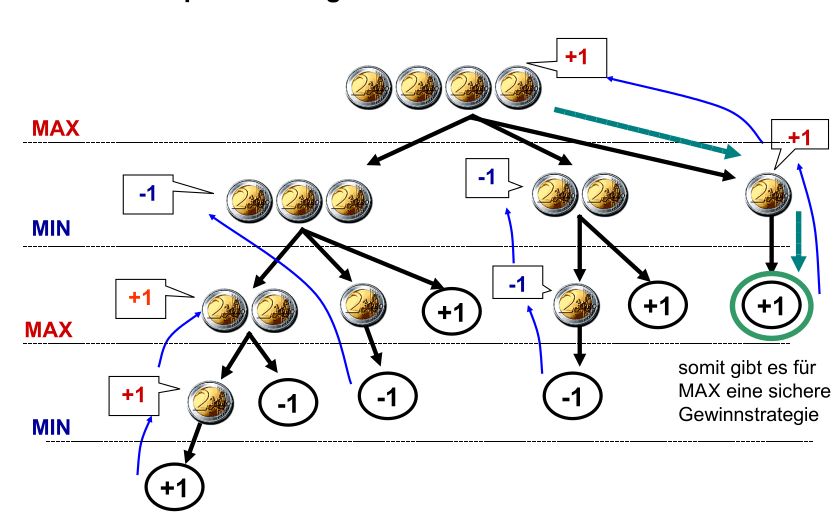
\includegraphics[width=0.8\textwidth]{figures/kap4/minmax-nimm.png}
    \caption{Bottom-up Bewertung der Knoten aus der Sicht von MAX}
    \label{fig:minmax-nimm-example}
\end{figure}

\subsection{Eigenschaften des MiniMax-Algorithmus}

Der Algorithmus ist vollst�ndig, wenn der Suchbaum endlich ist, und ist optimal, wenn gegen einen optimalen Spieler gespielt wird. Der Algorithmus hat ein Zeitbedarf von \(O(b^m)\) miz Suchtiefe \(m\) und Verzweigungsfaktor \(b\) und hat ein Platzbedarf von \(O(b*m)\). 

Dieser Algorithmus kann modifiziert werden, indem man die Tiefe des Baumes begrenzt (nur ein paar Runden vorausschaut) und den Nutzen einer Position mit einer guten Bewertungsfunktion absch�tzt.

\subsection{Verbesserung des MiniMax-Algorithmus durch Pruning}

Pruning, auch bekannt als \(\alpha\beta\)-Search oder \(\alpha\beta\)-Pruning, ist eine Idee, um die Effizienz des Minimax-Algorithmus zu verbessern, indem fr�hzeitig erkannt wird, welchem Zweig des Suchbaums nicht gefolgt werden muss.

Unter der Annahme, dass MIN und MAX jeweils den f�r sie optimalen Weg w�hlen, ist es m�glich fr�hzeitig zu erkennen, welche Verzweigungen des Suchbaums das Ergebnis nicht beeinflussen und daher nicht berechnet werden m�ssen. Unter Verwendung des Nimm-Beispiels k�nnen Pfade geschnitten werden, die ein schlechteres Ergebnis liefern als bereits erkundete Pfade.

\begin{figure}[H]
    \centering
    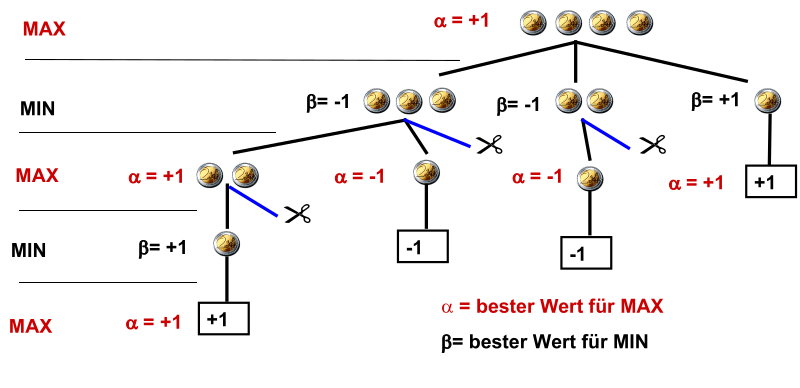
\includegraphics[width=0.8\textwidth]{figures/kap4/minxmax-pruning.png}
    \caption{Beschneiden des MinMax-Nimm-Beispiels}
    \label{fig:minmax-pruning-example}
\end{figure}

\subsection{Komplexit�t von MiniMax-Pruning}

Im schlimmsten Fall, wenn die Knoten in einer ung�nstigen Reihenfolge sind, dann ist es dasselbe wie bei einem normalen MiniMax. Im besten Fall k�nnte man die Mindestanzahl an Positionen berechnen lassen. Dies kann erreicht werden, indem die Reihenfolge der Bewegungen basierend auf der Effizienz der Bewegung neu geordnet wird. Zum Beispiel ist beim Schach das Schlagen einer Figur mit einem Turm oft vorteilhaft und sollte zuerst sequenziert werden.

\subsection{MiniMax in Spielen mit Zuf�lligkeit}

Die Zuf�lligkeit wird unter Verwendung zus�tzlicher Knoten im Suchbaum gehandhabt. F�r die Bewertung erh�lt jeder Zweig der Zufallsknoten den Durchschnitt aller m�glichen Zufallsergebnisse. 

\begin{figure}[H]
    \centering
    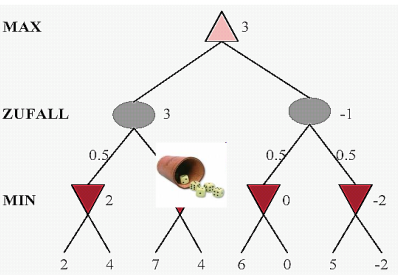
\includegraphics[width=0.6\textwidth]{figures/kap4/minmax-random.png}
    \caption{Zus�tzlicher Zufallknoten mit Mittelwert-Bewertung}
    \label{fig:minmax-random-example}
\end{figure}